
\documentclass[11pt]{article}

\usepackage[margin=0.82in]{geometry}
\usepackage[T1]{fontenc}
\usepackage[utf8]{inputenc}
\usepackage{lmodern}
\usepackage{microtype}
\usepackage{amsmath,amssymb}
\usepackage{booktabs,tabularx,array}
\usepackage{graphicx}
\usepackage{xcolor}
\usepackage{tikz}
\usetikzlibrary{positioning,arrows.meta,calc}
\usepackage{caption}
\usepackage{enumitem}
\usepackage[numbers,sort&compress]{natbib}
\usepackage{hyperref}
\usepackage{fancyhdr}
\usepackage[most]{tcolorbox}
\usepackage{titlesec}

\definecolor{aubblue}{HTML}{1F4E79}
\definecolor{softblue}{HTML}{EAF2F8}
\definecolor{softgreen}{HTML}{EAF6F1}
\definecolor{softgray}{HTML}{F4F6F7}
\definecolor{darkgreen}{HTML}{216A4A}

\hypersetup{
  colorlinks=true,
  linkcolor=aubblue,
  citecolor=aubblue,
  urlcolor=aubblue,
  pdftitle={BIOL 260 CDC14B circRNA-miRNA axis},
  pdfauthor={Jad Sawan}
}

\pagestyle{fancy}
\fancyhf{}
\lhead{BIOL 260 --- Take-Home Bioinformatics Exercise}
\rhead{CDC14B axis}
\cfoot{\thepage}
\setlength{\headheight}{14pt}

\titleformat{\section}{\large\bfseries\color{aubblue}}{\thesection}{0.6em}{}
\titleformat{\subsection}{\normalsize\bfseries\color{aubblue}}{\thesubsection}{0.5em}{}
\setlist[itemize]{leftmargin=1.25em,itemsep=2pt,topsep=3pt}
\setlist[enumerate]{leftmargin=1.55em,itemsep=3pt,topsep=3pt}

\newcommand{\mir}[1]{\textit{#1}}
\newcommand{\gene}[1]{\textit{#1}}
\newcommand{\circrna}[1]{\texttt{\detokenize{#1}}}

\begin{document}

\begin{center}
{\LARGE\bfseries\color{aubblue} Reconstructing a CDC14B-Derived circRNA--miRNA Regulatory Hypothesis in Breast Cancer}\\[0.7em]
{\large Jad Sawan}\\[0.2em]
BIOL 260 --- Section B2 \hfill September 2026
\end{center}

\vspace{0.35em}

\begin{tcolorbox}[colback=softblue,colframe=aubblue,boxrule=0.7pt,arc=2mm,title=Required answers at a glance]
\small
\begin{tabularx}{\linewidth}{>{\bfseries}p{0.26\linewidth}X}
Assigned gene & \gene{CDC14B} \\
Two circRNAs & \circrna{hsa_circ_0087640}, \circrna{hsa_circ_0087641} \\
Candidate miRNAs & \mir{hsa-miR-217-5p}, \mir{hsa-miR-106a-3p}, \mir{hsa-miR-136-5p} \\
Selected miRNA & \mir{hsa-miR-136-5p}; reported as reduced in breast cancer/TNBC \\
Kaplan--Meier result & METABRIC OS: HR $=0.84$ (95\% CI $0.69$--$1.02$), log-rank $p=0.081$ \\
TargetScan targets & \gene{ORC6}, \gene{XRCC2}, \gene{TFAP2C} \\
Final proposed axis & \gene{CDC14B} $\rightarrow$ \circrna{hsa_circ_0087640} $\dashv$ \mir{miR-136-5p} $\dashv$ \{\gene{ORC6}, \gene{XRCC2}, \gene{TFAP2C}\}
\end{tabularx}
\end{tcolorbox}

\section{Motivation: from a homework axis to a biological hypothesis}

The exercise asks for a gene $\rightarrow$ circRNA $\rightarrow$ miRNA $\rightarrow$ mRNA axis. The biological idea behind such an axis is that regulation does not occur only through proteins. RNA molecules can also influence one another by competing for binding partners. Circular RNAs (circRNAs), for example, can contain sequence motifs recognized by microRNAs (miRNAs). If a circRNA is expressed at sufficient abundance, is present in the correct cellular compartment, and physically binds a miRNA, it may reduce the amount of that miRNA available to repress its usual messenger-RNA (mRNA) targets. This type of proposed interaction is often described as miRNA ``sponging'' or competing-endogenous-RNA regulation \cite{Dudekula2016CircInteractome}.

The central question of this report is therefore not simply ``which names appear in a database?'' but rather:

\begin{quote}
\emph{Can a CDC14B-derived circRNA be used to formulate a biologically coherent, testable regulatory hypothesis involving a breast-cancer-relevant miRNA and downstream mRNA targets?}
\end{quote}

This distinction matters because a sequence match is only the first layer of evidence. A convincing computational hypothesis should also make sense in the disease context, be compatible with independent literature, and be interpreted honestly when clinical data do not provide statistically significant support.

\begin{tcolorbox}[colback=softgray,colframe=gray!65,boxrule=0.5pt,arc=2mm,title=Key terms used in the analysis]
\small
\begin{itemize}
    \item \textbf{circRNA:} a covalently closed RNA produced by \emph{back-splicing}, in which a downstream splice donor is joined to an upstream splice acceptor. The resulting back-splice junction is characteristic of the circular transcript.
    \item \textbf{miRNA:} a short regulatory RNA that guides a silencing complex toward complementary sites on other RNAs. Nucleotides 2--8 of the miRNA form the \textbf{seed}, a major determinant of target recognition.
    \item \textbf{miRNA response element:} a sequence on another RNA that is complementary to the miRNA seed. A predicted response element means the sequences are compatible; it does not prove binding inside a cell.
    \item \textbf{miRNA sponge:} an RNA proposed to bind and sequester a miRNA. True sponging requires more than a sequence match---expression level, localization, accessibility and stoichiometry also matter.
    \item \textbf{regulatory axis:} a compact model linking an upstream molecule to an intermediate regulator and downstream targets. Here it is a \emph{hypothesis-generating model}, not an experimentally established pathway.
\end{itemize}
\end{tcolorbox}

\section{Why CDC14B, and how the analysis was designed}

The assigned B2/J--O gene is \gene{CDC14B}. CDC14B is a dual-specificity phosphatase involved in cell-cycle control and DNA-damage checkpoint regulation. This makes it suitable for an exercise centered on cell-cycle and tumorigenesis events. In breast cancer, a meta-analysis of 5,218 tumors reported significant CDC14B downregulation and an association between lower CDC14B expression and poorer prognosis in triple-negative breast cancer (TNBC) \cite{Li2020CDC14B}.

Rather than choosing a familiar cancer miRNA first and then searching for evidence that supported it, the analysis proceeded from sequence to biology (Figure~\ref{fig:workflow}). This was meant to reduce cherry-picking. First, CDC14B-derived circRNAs were identified. Second, the mature circRNA sequence was scanned for canonical miRNA seed matches. Third, sequence-supported miRNAs were compared using independent breast-cancer evidence. Fourth, the assignment-required Kaplan--Meier analysis was performed. Finally, TargetScan predictions were inspected to propose downstream mRNA targets.

\begin{figure}[ht]
\centering
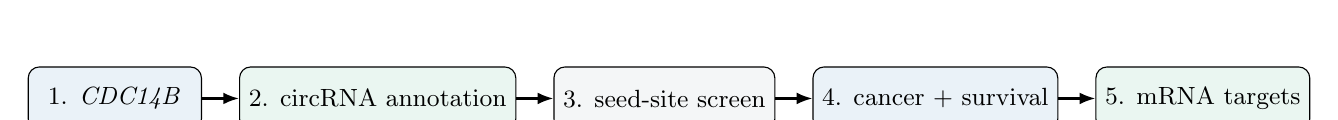
\begin{tikzpicture}[node distance=0.47cm and 0.47cm, every node/.style={font=\small}]
\node[draw,rounded corners,fill=softblue,minimum width=2.2cm,minimum height=0.8cm] (gene) {1. \gene{CDC14B}};
\node[draw,rounded corners,fill=softgreen,right=of gene,minimum width=2.55cm,minimum height=0.8cm] (circ) {2. circRNA annotation};
\node[draw,rounded corners,fill=softgray,right=of circ,minimum width=2.55cm,minimum height=0.8cm] (mir) {3. seed-site screen};
\node[draw,rounded corners,fill=softblue,right=of mir,minimum width=2.55cm,minimum height=0.8cm] (clin) {4. cancer + survival};
\node[draw,rounded corners,fill=softgreen,right=of clin,minimum width=2.45cm,minimum height=0.8cm] (tar) {5. mRNA targets};
\draw[-{Latex[length=2mm]},thick] (gene) -- (circ);
\draw[-{Latex[length=2mm]},thick] (circ) -- (mir);
\draw[-{Latex[length=2mm]},thick] (mir) -- (clin);
\draw[-{Latex[length=2mm]},thick] (clin) -- (tar);
\end{tikzpicture}
\caption{Sequence-first evidence-integration workflow. The purpose of the additional computational steps was not to make the homework larger, but to make the final choice less dependent on a single database lookup.}
\label{fig:workflow}
\end{figure}

\section{Step 1: identifying CDC14B-derived circular RNAs}

Two CDC14B-derived circRNAs were retained (Table~\ref{tab:circs}). \circrna{hsa_circ_0087640} was used for downstream sequence screening because TransCirc provides its full mature sequence and cross-references the record to circBase; \circrna{hsa_circ_0087641} is independently annotated in circBase as a CDC14B-derived circRNA. TransCirc and circBase are established circRNA resources \cite{Huang2021TransCirc,Glazar2014circBase}.

\begin{table}[ht]
\centering
\caption{CDC14B-derived circRNAs used for the exercise.}
\label{tab:circs}
\begin{tabularx}{\linewidth}{@{}l l X@{}}
\toprule
\textbf{circRNA} & \textbf{Host gene} & \textbf{Why it was retained} \\
\midrule
\circrna{hsa_circ_0087640} & CDC14B & Primary candidate; a complete mature sequence was available, allowing direct sequence-level miRNA-site screening. \\
\circrna{hsa_circ_0087641} & CDC14B & Independent CDC14B circRNA annotation used to satisfy the requirement for two predicted/annotated circular RNAs. \\
\bottomrule
\end{tabularx}
\end{table}

The distinction between a host gene and its circRNA is important. A circRNA derived from CDC14B is not equivalent to the linear CDC14B mRNA: back-splicing creates a different RNA molecule with its own junction and potentially different regulatory interactions. Therefore, downstream miRNA prediction was performed on the mature circRNA sequence rather than inferred simply from the host-gene name.

\section{Step 2: predicting miRNAs from the circRNA sequence}

\subsection{Why a custom sequence scan was used}

The CircInteractome URL supplied in the exercise returned a page-not-found error during the analysis. Instead of replacing the requested method with an unrelated database, the intended sequence logic was reconstructed programmatically from the mature \circrna{hsa_circ_0087640} sequence. CircInteractome uses TargetScan-style miRNA target-site logic, so the scan searched for the three canonical seed classes emphasized in TargetScan \cite{Dudekula2016CircInteractome,Agarwal2015TargetScan}:

\begin{itemize}
    \item \textbf{8mer:} complementarity to miRNA nucleotides 2--8 together with an additional adenosine opposite miRNA position 1;
    \item \textbf{7mer-m8:} complementarity to miRNA nucleotides 2--8;
    \item \textbf{7mer-A1:} complementarity to nucleotides 2--7 plus the additional adenosine.
\end{itemize}

Because the RNA is circular, the script also searched across the back-splice junction. This prevents the computational representation of a circular molecule as an ordinary linear string from missing a site that spans the end and beginning of the written sequence.

\subsection{How candidates were ranked}

The mature-miRNA reference was miRBase v22.1. The initial scan found 406 mature miRNAs with at least one canonical site. Many miRNAs, however, share the same nucleotides 2--8 and therefore generate the same seed-based sequence hypothesis. These were collapsed into 309 seed families before ranking.

For transparency, the following simple score was used:
\[
S_{\mathrm{seed}}
=
3N_{8\mathrm{mer}}
+
2N_{7\mathrm{mer-m8}}
+
N_{7\mathrm{mer-A1}}.
\]
The score is \emph{not} a binding-energy model and is not presented as a validated biological metric. It is only a reproducible way to rank canonical site architectures, giving more weight to the stronger canonical classes.

Three candidates were retained after combining sequence support with independent breast-cancer relevance (Table~\ref{tab:mirs}). This extra screening step is why the final answer is not simply the top sequence hit.

\begin{table}[ht]
\centering
\caption{Three prioritized miRNA candidates predicted from \circrna{hsa_circ_0087640}.}
\label{tab:mirs}
\begin{tabularx}{\linewidth}{@{}l c c c X@{}}
\toprule
\textbf{miRNA} & \textbf{8mer} & \textbf{7mer-m8} & $\mathbf{S_{seed}}$ & \textbf{Why it remained biologically interesting} \\
\midrule
\mir{hsa-miR-217-5p} & 2 & 0 & 7 & Strongest sequence candidate; independently reported as reduced in breast cancer and tumor-suppressive through MTDH/NF-$\kappa$B/EMT regulation \cite{Yang2022miR217}. \\
\mir{hsa-miR-106a-3p} & 1 & 1 & 5 & Independent work links it to mammary epithelial plasticity and increased tumoroid initiation in a 3D human mammary model \cite{Robert2026miR106a}. \\
\mir{hsa-miR-136-5p} & 1 & 1 & 5 & Reported as reduced in TNBC and experimentally involved in breast-cancer circRNA sponge axes \cite{Yan2016miR136,Zhong2021circERBB2}. \\
\bottomrule
\end{tabularx}
\end{table}

\subsection{Why miR-136-5p was chosen for the formal homework axis}

The strongest sequence-only candidate was miR-217-5p. However, the assignment also requires a Kaplan--Meier analysis in the breast-cancer miRNA framework, and among the three finalists only the older identifier \mir{hsa-miR-136} was available in the assignment-specified METABRIC cohort in the current KM Plotter interface. miR-136-5p was therefore selected because it satisfied \emph{all} required layers: canonical circRNA seed support, independent breast-cancer relevance, prior evidence that it can participate in circRNA-sponging mechanisms in breast tissue, and availability for the required METABRIC survival analysis.

This should not be interpreted as proof that miR-136-5p is the uniquely best binder of \circrna{hsa_circ_0087640}. Rather, it is the strongest candidate that could be followed consistently through every step of the exercise.

The legacy miRCancer interface specified in the homework was not reliably accessible during the analysis, so direction of dysregulation was verified from primary literature. miR-136 has been reported as reduced in TNBC, and restoration of miR-136 suppressed invasion and metastasis \cite{Yan2016miR136}. In HER2-positive breast cancer, circ-ERBB2 was experimentally shown to sponge miR-136-5p and relieve repression of \gene{TFAP2C}, establishing that this miRNA can participate in the type of circRNA-mediated regulatory mechanism hypothesized here \cite{Zhong2021circERBB2}.

\section{Step 3: what the Kaplan--Meier analysis tests}

A Kaplan--Meier curve estimates the probability of remaining alive over time. Here, patients were divided into \textbf{high-} and \textbf{low-miR-136 expression} groups using the median expression level. The two survival curves were then compared.

Two statistics are especially important:

\begin{itemize}
    \item The \textbf{hazard ratio (HR)} compares the estimated instantaneous risk of death between the two expression groups. With the KM Plotter orientation used here, an HR below 1 indicates lower estimated hazard in the high-expression group.
    \item The \textbf{95\% confidence interval and log-rank $p$-value} indicate the uncertainty around that association. If the confidence interval includes 1 and $p>0.05$, the result should not be called statistically significant.
\end{itemize}

The Kaplan--Meier Plotter/miRpower framework was run using METABRIC, overall survival (OS), a median expression split, unrestricted follow-up, and no subtype or treatment restrictions \cite{Lanczky2016miRpower}. The database recognized the older label \mir{hsa-miR-136}; the mature-arm interpretation used elsewhere in the report is \mir{hsa-miR-136-5p}.

The low-expression group contained 637 patients and the high-expression group 625 patients ($N=1262$). Higher miR-136 expression produced an HR of $0.84$ (95\% CI $0.69$--$1.02$), with a log-rank $p=0.081$. The point estimate therefore suggests approximately 16\% lower estimated hazard in the high-expression group, which is directionally compatible with a tumor-suppressive interpretation. However, the confidence interval includes 1 and $p=0.081>0.05$. The correct conclusion is therefore \textbf{a non-significant trend}, not a validated prognostic effect.

\begin{figure}[ht]
\centering
\includegraphics[width=0.58\linewidth]{figures/km_mir136_metabric.pdf}
\caption{Kaplan--Meier overall-survival analysis for \mir{hsa-miR-136} in METABRIC. Median split, no clinical subtype restrictions. High expression: $n=625$; low expression: $n=637$; HR $=0.84$ (95\% CI $0.69$--$1.02$); log-rank $p=0.081$.}
\label{fig:km}
\end{figure}

\section{Step 4: predicting downstream mRNA targets with TargetScan}

A miRNA response element on a circRNA suggests that the circRNA \emph{could} bind the miRNA. The other half of the proposed axis asks what that miRNA might normally repress. TargetScan predicts miRNA target sites in mRNAs using seed matching together with sequence-context features that influence targeting efficacy \cite{Agarwal2015TargetScan}.

TargetScan predictions were queried through the multiMiR R package \cite{Ru2014multiMiR}; the local database metadata reported TargetScan version 8.0 (September 2021). The top 20\% of predictions were retained as a pre-specified filter so that genes were not selected from an arbitrarily large prediction universe only because they happened to fit the expected story. After collapsing duplicate transcript/site records, the miR-136-5p prediction set contained 891 unique genes.

TargetScan reports a context-type score in which more-negative values generally correspond to stronger predicted repression. Importantly, this is still a \emph{prediction score}: a negative value does not mean that the target has been experimentally validated.

Three genes were selected from the actual TargetScan output because they connect naturally to cell-cycle, DNA-repair and breast-cancer biology (Table~\ref{tab:targets}).

\begin{table}[ht]
\centering
\caption{Representative downstream TargetScan predictions for \mir{hsa-miR-136-5p}.}
\label{tab:targets}
\begin{tabularx}{\linewidth}{@{}l c X@{}}
\toprule
\textbf{Target} & \textbf{TargetScan score} & \textbf{Why the target is biologically interpretable} \\
\midrule
\gene{ORC6} & $-0.558$ & Origin-recognition-complex subunit required for DNA-replication initiation/cell division; high ORC6 expression has been associated with increased proliferation and poor breast-cancer outcome \cite{Ibrahim2024ORC6}. \\
\gene{XRCC2} & $-0.476$ & RAD51 paralog involved in homologous-recombination repair of DNA double-strand breaks \cite{Andreassen2019XRCC2}. \\
\gene{TFAP2C} & $-0.374$ & Breast-cancer transcription factor; independently validated as a direct miR-136-5p target in a circ-ERBB2/miR-136-5p/TFAP2C axis \cite{Zhong2021circERBB2}. \\
\bottomrule
\end{tabularx}
\end{table}

\section{Putting the pieces together}

The proposed model is:

\begin{tcolorbox}[colback=softgreen,colframe=darkgreen,boxrule=0.9pt,arc=2mm]
\centering
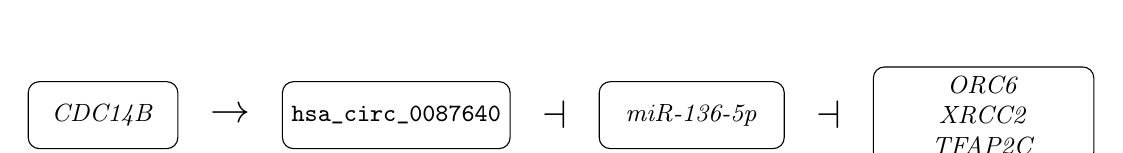
\begin{tikzpicture}[every node/.style={font=\small},node distance=0.42cm]
\node[draw,rounded corners,fill=white,minimum width=1.9cm,minimum height=0.85cm] (g) {\gene{CDC14B}};
\node[right=0.28cm of g,font=\Large] (a1) {$\rightarrow$};
\node[draw,rounded corners,fill=white,right=0.28cm of a1,minimum width=2.8cm,minimum height=0.85cm] (c) {\circrna{hsa_circ_0087640}};
\node[right=0.28cm of c,font=\Large] (a2) {$\dashv$};
\node[draw,rounded corners,fill=white,right=0.28cm of a2,minimum width=2.35cm,minimum height=0.85cm] (m) {\mir{miR-136-5p}};
\node[right=0.28cm of m,font=\Large] (a3) {$\dashv$};
\node[draw,rounded corners,fill=white,right=0.28cm of a3,minimum width=2.8cm,minimum height=0.85cm,align=center] (t) {\gene{ORC6}\\\gene{XRCC2}\\\gene{TFAP2C}};
\end{tikzpicture}

\vspace{0.55em}
\small $\rightarrow$: circRNA derived from host gene; $\dashv$: proposed sequestration or miRNA-mediated repression.
\end{tcolorbox}

The logic of the hypothesis is as follows. CDC14B can generate \circrna{hsa_circ_0087640}. The mature circRNA sequence contains canonical sites compatible with miR-136-5p binding. If this interaction occurs in breast cells and the circRNA is sufficiently abundant, the circRNA could reduce the effective availability of miR-136-5p. Since miRNAs normally repress compatible mRNA targets, reduced free miR-136-5p could in turn relieve repression of some downstream transcripts, including predicted targets such as \gene{ORC6}, \gene{XRCC2} and \gene{TFAP2C}.

This is why the two inhibitory symbols in the axis should not be read as direct experimental facts. They encode the regulatory logic being tested: a putative circRNA $\dashv$ miRNA interaction followed by miRNA $\dashv$ mRNA repression.

\section{What the extended computational analysis added}

The extra analysis was useful mainly as a \textbf{quality-control layer}. It did not create a statistically significant survival result, nor was it intended to do so. Instead, it answered three questions that a simple database worksheet would leave unresolved.

First, it showed that sequence rank and disease relevance are not the same thing. miR-217-5p was the strongest sequence-derived candidate, while another highly ranked family, miR-5197-5p, had much weaker breast-cancer support. This helped prevent a purely sequence-driven choice.

Second, the analysis forced the candidate choice to be explicit. miR-136-5p was not chosen because it had the largest score; it was chosen because it combined sequence support, breast-cancer evidence, prior circRNA-sponging precedent, and availability in METABRIC for the required clinical step.

Third, an exploratory GO analysis was used as a robustness check rather than as a source of a dramatic story. Several apparently interesting pathway terms appeared under an all-human-gene background, but those signals were not robust when the background was changed to the union of TargetScan-predicted genes. For that reason, no pathway-level mechanism was claimed from GO enrichment. In other words, the additional computation mainly helped identify where the evidence \emph{stops}.

\section{Limitations and what would be needed experimentally}

The proposed axis remains computational. Four limitations are especially important:

\begin{enumerate}
    \item The CircInteractome interface linked in the exercise was unavailable, so its intended sequence-prediction logic was reconstructed rather than copied directly from the website.
    \item A seed match does not prove miRNA sponging. A true sponge mechanism would require appropriate expression, localization and molecular stoichiometry in breast cells.
    \item TargetScan predicts potential miRNA--mRNA interactions but does not demonstrate functional repression in this specific CDC14B context.
    \item The METABRIC result is directionally favorable but statistically non-significant; it should not be described as a prognostic biomarker result.
\end{enumerate}

A logical experimental follow-up would therefore include junction-specific quantification of \circrna{hsa_circ_0087640}, confirmation of its subcellular localization, AGO2/RNA-pull-down or luciferase assays to test the circRNA--miR-136-5p interaction, and perturbation experiments to determine whether changing the circRNA or miRNA alters the predicted downstream targets.

\section{Conclusion}

The homework requirements can be summarized by the proposed axis
\[
\boxed{
\gene{CDC14B}
\rightarrow
\circrna{hsa_circ_0087640}
\dashv
\mir{miR-136-5p}
\dashv
\{\gene{ORC6},\gene{XRCC2},\gene{TFAP2C}\}
}.
\]

The main conclusion is deliberately modest: this is a reproducible and biologically motivated \emph{hypothesis}, not an experimentally established pathway. The sequence data make miR-136-5p a plausible interaction partner for the CDC14B-derived circRNA; independent literature supports its relevance to breast cancer; TargetScan supplies plausible downstream targets; and METABRIC shows a directionally favorable but non-significant survival trend. Together, these layers justify the axis as a candidate for experimental testing while also defining the limits of the computational evidence.


\begin{thebibliography}{99}
\small

\bibitem{Li2020CDC14B}
J.-D. Li, G. Chen, M. Wu, Y. Huang, and W. Tang.
Downregulation of CDC14B in 5218 breast cancer patients: A novel prognosticator for triple-negative breast cancer.
\textit{Mathematical Biosciences and Engineering}, 17(6):8152--8181, 2020.
\href{https://doi.org/10.3934/mbe.2020414}{doi:10.3934/mbe.2020414}.

\bibitem{Dudekula2016CircInteractome}
D. B. Dudekula, A. C. Panda, I. Grammatikakis, S. De, K. Abdelmohsen, and M. Gorospe.
CircInteractome: A web tool for exploring circular RNAs and their interacting proteins and microRNAs.
\textit{RNA Biology}, 13(1):34--42, 2016.
\href{https://doi.org/10.1080/15476286.2015.1128065}{doi:10.1080/15476286.2015.1128065}.

\bibitem{Glazar2014circBase}
P. Gla\v{z}ar, P. Papavasileiou, and N. Rajewsky.
circBase: a database for circular RNAs.
\textit{RNA}, 20(11):1666--1670, 2014.
\href{https://doi.org/10.1261/rna.043687.113}{doi:10.1261/rna.043687.113}.

\bibitem{Huang2021TransCirc}
W. Huang, Y. Ling, S. Zhang, Q. Xia, R. Cao, X. Fan, Z. Fang, Z. Wang, and G. Zhang.
TransCirc: an interactive database for translatable circular RNAs based on multi-omics evidence.
\textit{Nucleic Acids Research}, 49(D1):D236--D242, 2021.
\href{https://doi.org/10.1093/nar/gkaa823}{doi:10.1093/nar/gkaa823}.

\bibitem{Agarwal2015TargetScan}
V. Agarwal, G. W. Bell, J.-W. Nam, and D. P. Bartel.
Predicting effective microRNA target sites in mammalian mRNAs.
\textit{eLife}, 4:e05005, 2015.
\href{https://doi.org/10.7554/eLife.05005}{doi:10.7554/eLife.05005}.

\bibitem{Ru2014multiMiR}
Y. Ru et al.
The multiMiR R package and database: integration of microRNA-target interactions along with their disease and drug associations.
\textit{Nucleic Acids Research}, 42(17):e133, 2014.
\href{https://doi.org/10.1093/nar/gku631}{doi:10.1093/nar/gku631}.

\bibitem{Yan2016miR136}
M. Yan, X. Li, D. Tong, C. Han, R. Zhao, Y. He, and X. Jin.
miR-136 suppresses tumor invasion and metastasis by targeting RASAL2 in triple-negative breast cancer.
\textit{Oncology Reports}, 36(1):65--71, 2016.
\href{https://doi.org/10.3892/or.2016.4767}{doi:10.3892/or.2016.4767}.

\bibitem{Zhong2021circERBB2}
J.-X. Zhong et al.
Circular RNA circ-ERBB2 promotes HER2-positive breast cancer progression and metastasis via sponging miR-136-5p and miR-198.
\textit{Journal of Translational Medicine}, 19:455, 2021.
\href{https://doi.org/10.1186/s12967-021-03114-8}{doi:10.1186/s12967-021-03114-8}.

\bibitem{Lanczky2016miRpower}
A. L\'anczky, A. Nagy, G. Bottai, G. Munk\'acsy, A. Szab\'o, L. Santarpia, and B. Gy\H{o}rffy.
miRpower: a web-tool to validate survival-associated miRNAs utilizing expression data from 2178 breast cancer patients.
\textit{Breast Cancer Research and Treatment}, 160(3):439--446, 2016.
\href{https://doi.org/10.1007/s10549-016-4013-7}{doi:10.1007/s10549-016-4013-7}.

\bibitem{Ibrahim2024ORC6}
A. Ibrahim et al.
Novel 2 Gene Signatures Associated With Breast Cancer Proliferation: Insights From Predictive Differential Gene Expression Analysis.
\textit{Modern Pathology}, 37(2):100403, 2024.
\href{https://doi.org/10.1016/j.modpat.2023.100403}{doi:10.1016/j.modpat.2023.100403}.

\bibitem{Andreassen2019XRCC2}
P. R. Andreassen and H. Hanenberg.
XRCC2 (X-ray repair cross complementing 2).
\textit{Atlas of Genetics and Cytogenetics in Oncology and Haematology}, 23(1):1--7, 2019.
\href{https://doi.org/10.4267/2042/69759}{doi:10.4267/2042/69759}.

\bibitem{Robert2026miR106a}
J. Robert et al.
A miRNA screen reveals a transcriptional network controlling the initiation of mammary organoids.
\textit{The FEBS Journal}, 293(11):3228--3258, 2026.
\href{https://doi.org/10.1111/febs.70397}{doi:10.1111/febs.70397}.

\bibitem{Yang2022miR217}
L. Yang et al.
miR-217-5p suppresses epithelial-mesenchymal transition and the NF-$\kappa$B signaling pathway in breast cancer via targeting of metadherin.
\textit{Oncology Letters}, 23(5):162, 2022.
\href{https://doi.org/10.3892/ol.2022.13282}{doi:10.3892/ol.2022.13282}.

\end{thebibliography}
\end{document}
